\documentclass[12pt]{article}
\usepackage[left=1in, right=1in, top=1in, bottom=1in]{geometry}
\usepackage{graphicx}
\newtheorem{theorem}{Theorem}[section]
\usepackage{amsmath}
\usepackage{amssymb}
\usepackage{amsthm}
\theoremstyle{plain}
\newtheorem*{theorem*}{Theorem}
\usepackage{hyperref}
\usepackage{amsmath}
\usepackage{dsfont}
\usepackage{tikz}
\usetikzlibrary{automata,positioning,arrows}
\usepackage{babel}
\usepackage{calc}
\usepackage{graphicx}
\usepackage{caption}
\usepackage{lipsum}

\begin{document}
\begin{center}
\section*{Introduction to Machine Learning Section 4}
\subsubsection*{Saar Barak}
\end{center}
\subsubsection*{ 1.  SVM with multiple classes. }
Define the following multiclass SVM problem:
\[f(w_1,\dots w_k)=\frac{1}{n}\sum^n_{i=1}\ell(w_1,\dots w_k,x_i,y_i)=\frac{1}{n}\sum^n_{i=1}
\underset{j\in [K]}{\text{max}}(w_j \cdot x_i -w_{y_i}\cdot x_i + \mathds{1}(j\neq y_i) )
\]
First lets notice that if $i=j$ then f is sum of zeros, hence $f$ is non-negative function and we assume that the data is linearly separable, 
we can consider $\mathbf{w^*}=(w_1^*,\dots w_k^*) $ to be the actual separator of the data. its will be  sufficient to see  that.
after plug-in $\mathbf{w^*}$ any minimizer will lead $f$ to 0 errors. so we just need to make sure that for any update s.t $\mathds{1}(y_i\neq j)$.  will lead  $f \mapsto 0$
  \[w_j \cdot x_i -w_{y_i}\cdot x_i + \mathds{1}(j\neq y_i)=x_i(w_j-w_{y_i})+\mathds{1}
  \]
$x_iw_j^*=M_j$ is the support vector of the data for some $y$. according to the max margin hyperplane property the the true separator $\mathbf{w^*}$ maximize the minimum distance for any $y$. and now we just need to see that for any $j\in [K]/y_i$ 
  \[x_iw_j-x_iw_{y_i}=\frac{1}{M}(x_i(w_j^*-w_{y_i}^*)=\frac{-1}{M}(x_i(w_{y_i}^*-w_j^*))\leq \frac{-1}{M}\text{Min}_j(x_i(w_{y_i}^*-w_j^*))\leq -1
  \]
  since any other margin will be $\geq$  $M$.
\\ Hence after the  $multiclass-hinge-loss$ find the actual max margin hyperplane any minimizer apply on $f$ will lead to 0 errors.
\subsubsection*{ 2.  Soft-SVM. }
Consider the soft-SVM problem with seperable data:

\[\begin{array}{ll}
\underset{\mathbf{w},\xi}{\text{min}} & 0.5||\mathbf{w}||^2 + C\sum^n_{i=1}\xi_i \\

\text{ s.t } \forall i: & y_i\mathbf{w\cdot x}_i \ge 1-\xi_i \\
&\xi_i \ge 0.
\end{array}\]
Let $\mathbf{w}^\star$ be the solution of\textbf{ hard SVM}, and let $\mathbf{w}',\xi '$ be   solution for the \textbf{ soft SVM}. since $\mathbf{w}^\star$ feasible  solution for the problem.  I claim that the  following holds for  $C\geq||\mathbf{w}^\star||^2$
\[\frac{1}{2}||\mathbf{w'}||^2+||\mathbf{w}^\star||^2||\xi'||\leq\frac{1}{2}||\mathbf{w'}||^2+C||\xi'||\leq\frac{1}{2}||\mathbf{w}^\star||^2\Rightarrow \frac{1}{2}||\mathbf{w'}||^2\leq ||\mathbf{w}^\star||^2(\frac{1}{2}-||\xi'||)
\]
Since all non negative any minimizer of the problem will lead to $\sum_i \xi < 1$. we can notice that for any $\xi_i$
\[0\leq \frac{|1-\xi_i|}{||w||}<1
\] 
Any point  
$x_i$
 which is within the margin or is located in the other side of the separating hyperplane, but none of them cross the separating hyperplane hence the data is separable
\subsubsection*{ 3.  Separability using polynomial kernel. }
Let $x_1,\dots x_n \in \mathbb{R}$e distinct real
numbers, and let $q \geq n$ be an integer.
for separable data hard-SVM yield zero training errors. lets write the  polynomial kernel in binomial form
\[
(x,x')=(1+xx')^q=\sum^q_{k=0}\binom{q}{k}(xx')^k=\sum^q_{k=0}x^k\sqrt{\binom{q}{k}}x'^k\sqrt{\binom{q}{k}}
\] 
 Multiply each row of the Vandernow matrix with the constant from the binomial above.
\[
\begin{pmatrix}
x_1^0 & x_1^1 & x_2^2 & \cdots  & x_1^q \\
x_2^0 & x_2^1 & x_2^2 & \cdots  & x_2^q\\
\vdots &  &  & &    \\
x_q^0 & x_q^1 & x_q^2 & \cdots  & x_q^q
\end{pmatrix}
\Rightarrow
\begin{pmatrix}
x_1^0\sqrt{\binom{q}{0}} & x_1^1\sqrt{\binom{q}{1}} & x_2^2\sqrt{\binom{q}{2}} & \cdots  & x_1^q\sqrt{\binom{q}{q}} \\
x_1^0\sqrt{\binom{q}{0}} & x_1^1\sqrt{\binom{q}{1}} & x_2^2\sqrt{\binom{q}{2}} & \cdots  & x_1^q\sqrt{\binom{q}{q}}\\
\vdots &  &  & &    \\
x_1^0\sqrt{\binom{q}{0}} & x_1^1\sqrt{\binom{q}{1}} & x_2^2\sqrt{\binom{q}{2}} & \cdots  & x_1^q\sqrt{\binom{q}{q}}\end{pmatrix}
\]
Hence the binomial form can get by the inner proudact,  and $K_S$ the kernel matrix  $K(x_i,x_j)=\phi(x_i)\phi(x_j)$. using the fact that Vandernow matrix is rank $n$ the lemma holds here,  The hard-SVM yield zero training errors.
\subsubsection*{ 4.   Expressivity of ReLU networks. }
\begin{list}{•}{\textbf{4(a)}}
\item If $x\geq 0\Rightarrow x=\max\{0,x\},0=\max\{0,-x\}\Rightarrow x=x-0=\max\{0,x\}-\max\{0,-x\}$\\
If $x< 0\Rightarrow 0=\max\{0,x\},-x=\max\{0,-x\}\Rightarrow x-x=0 $\\$\Rightarrow x+\max\{0,-x\}=\max\{0,x\}\Rightarrow x= \max\{0,x\}-\max\{0,-x\} $
\item If $x\geq 0 ,-x\leq 0\Rightarrow x\geq -x \Rightarrow \max(x,-x)=x=|x|$
\\If $x< 0 ,-x> 0\Rightarrow x< -x \Rightarrow \max(x,-x)=-x=|x|$ 
\item \begin{eqnarray}
\frac{x_1+x_2}{2}+\frac{|x_1-x_2|}{2} &=& \frac{(x_1+x_2+\max(x_1-x_2,x_2-x_1))}{2} \\
&=& \frac{1}{2}(\max(x_1-x_2+x_1+x_2,x_2-x_1+x_1+x_2)) \\
&=& \frac{1}{2}(\max(2x_1,2x_2)) \\
&=& \max(x_1,x_2)
\end{eqnarray}
\end{list}

\subsubsection*{4(b)}
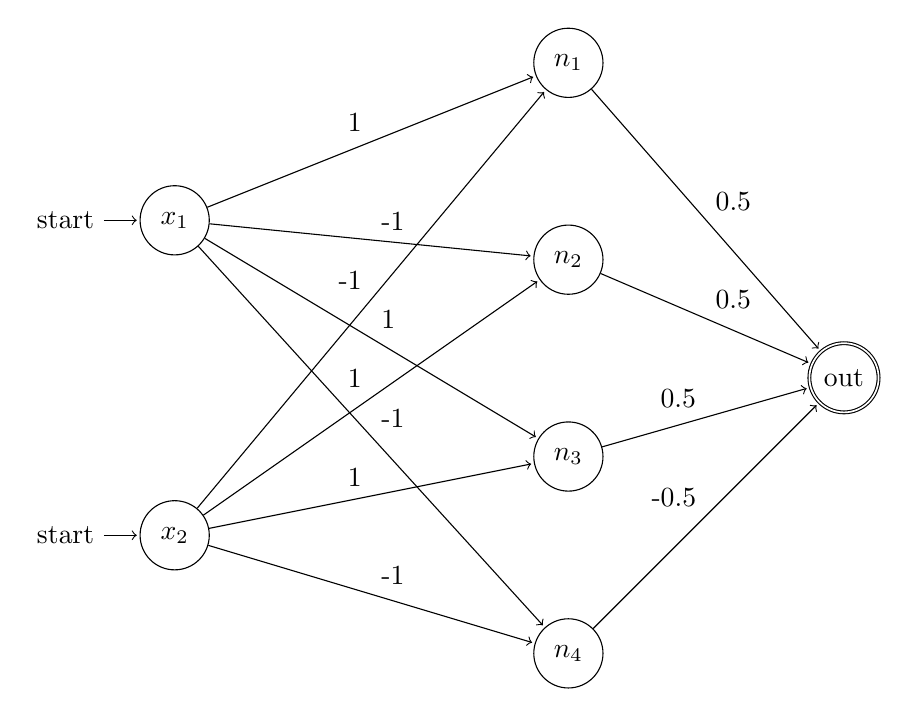
\begin{tikzpicture}[shorten >=1pt,node
 distance=2.5cm,on grid,auto] 
\node[state,initial] (q_0)   {$x_1$}; 
\node[state] (q_2) [state] at (5,2) {$n_1$}; 
\node[state] (q_3) [ below=of q_2] {$n_2$}; 
\node[state] (q_4) [ below=of q_3] {$n_3$}; 
\node[state] (q_5) [ below=of q_4] {$n_4$}; 
\node[state,initial]at (0,-4)  (q_1) {$x_2$}; 
    \node[state,accepting]at (8.5,-2)  (out) {out}; 

    \path[->] 
    (q_0) edge  node {1} (q_2)
    (q_1) edge  node {-1} (q_2)
    (q_0) edge  node {-1} (q_3)
    (q_1) edge  node {1} (q_3)
    (q_0) edge  node {1} (q_4)
    (q_1) edge  node {1} (q_4)
     (q_0) edge  node {-1} (q_5)
    (q_1) edge  node {-1} (q_5)
    (q_2) edge  node {0.5} (out)
    (q_3) edge  node {0.5} (out)
    (q_4) edge  node {0.5} (out)
    (q_5) edge  node {-0.5} (out)
;
\end{tikzpicture}\\
$n_1=\max \{x_1-x_2,0\},n_2=\max \{x_2-x_1,0\},n_3=\max \{x_1+x_2,0\},n_4=\max \{-x_1-x_2,0\}$
\\ (*) We could achieve same result with 3 neutrons since $\max \{x_1,x_2\}=\max\{x_1-x_2,0\}+x_2$

\subsubsection*{ 5.  Implementing boolean functions using ReLU networks. }
Consider n
boolean input variables $x_1,x_2\dots,x_n\in \{0,1\}$, lets construct a neural network
with ReLU activations, which implements the AND function:
\[f(x_1,x_2\dots,x_n)=x_1\wedge x_2\wedge\dots \wedge x_n
\] we can consider the $f$ as :
\[f(x_1,x_2\dots,x_n)=\max\{-n+1+\sum^n_{i=1} x_i,0\}
\]
Hence we can built ReLU networks with one hidden layer, and constant extra input $\hat{x}=1$, and the weight function will be 
\[  w(x_i)=1 \text{ for } 0\le i\le n \text{ and } w(\hat{x})=n-1
\]
By connecting all the inputs to single neuron we get the $\max \{\sum x_i,0\}$ and connecting  the constant $\hat{x_i}$ to it as well will give us the AND function $$\max \{\hat{x}(n-1)+\sum x_i,0\}$$
\pagebreak
\begin{center}
\subsection*{Programming Assignment. }
\subsubsection*{ SVM }
\end{center}
\noindent \begin{minipage}{0.5\textwidth}
\vspace{1cm}
\includegraphics[width=\textwidth]{plot 4.1.png}
\captionof{figure}{\textbf{Homogeneous} polynomial
kernel.}
\label{fig:1}
\end{minipage}
\hspace{0.05\textwidth}
\begin{minipage}{0.4\textwidth}
Here, the polynomial
kernel of degree 2 fits the data better, since the data is cycle shape shape, and the kernel trick need 2 degree for separate the hyperplane.
\end{minipage}


\begin{minipage}{0.4\textwidth}
We can see here better fit of of the right-hand side module, the Independent term in kernel function give the needed correction , but still degree 2 polynomial fits here better
\end{minipage}
\hspace{0.05\textwidth}
\noindent \begin{minipage}{0.5\textwidth}
\vspace{1cm}
\includegraphics[width=\textwidth]{plot 4.2.png}
\captionof{figure}{\textbf{Non-Homogeneous} polynomial
kernel.}
\label{fig:2}
\end{minipage}
\noindent \begin{minipage}{0.5\textwidth}
\vspace{1cm}
\includegraphics[width=\textwidth]{plot 4.3.png}
\captionof{figure}{polynomial
kernel and RBF kernel.}
\label{fig:3}
\end{minipage}
\hspace{0.05\textwidth}
\begin{minipage}{0.4\textwidth}
RBF kernel generalize better on the noisy data 
since its can separate the data in higher dimention then the polynomial
kernel, that become more "elliptic" to cover the noise data
\end{minipage}

\includegraphics[width=\textwidth]{crosskernal.png}
\captionof{figure}{\textbf{RBF kernel} 
 with different $\gamma$ values }
\label{fig:4}
 \vspace{0.4cm}
 
\subsection*{Neural Networks. }
\noindent \begin{minipage}{0.5\textwidth}
\vspace{0.4cm}
\includegraphics[width=\textwidth]{plot 4.4.png}
\captionof{figure}{}
\label{fig:nature}
\end{minipage}
\hspace{0.02\textwidth}
\begin{minipage}{0.5\textwidth}
\vspace{0.4cm}
\includegraphics[width=\textwidth]{plot 4.5.png}
\captionof{figure}{}
\label{fig:nature}
\end{minipage}

\begin{center}
\includegraphics[width=100mm]{plot 4.6.png}
\captionof{figure}{}
\label{fig:nature}
\end{center}




\begin{minipage}{0.6\textwidth}
From the plots we can learn that the best value for the learning rate is 0.1, while using larger value at any step we might get far away from the optimal minimizer, and while using smaller value we proses in less effective  way and loosing information.\end{minipage}
\hspace{0.05\textwidth}
\begin{minipage}{0.4\textwidth}
\vspace{0.4cm}
\includegraphics[width=\textwidth]{plot 4.7.jpg}
\captionof{figure}{accuracy in the final epoch}
\label{fig:nature}
\end{minipage}

\end{document}
